\chapter{Additional Theorems and Proofs}

\begin{theorem}[Sums of Independent Poisson Point Processes]\label{thm:sum_ppp}
    Given independent Poisson point processes $\{\N_1(t)\}_{t\geq0},
        \{\N_2(t)\}_{t\geq0}, \dots,  \{\N_n(t)\}_{t\geq0},$ with intensities
    $\lambda_1, \lambda_2, \dots, \lambda_n,$
    $$\{\N(t)\}_{t\geq0} := \{\N_1(t) + \N_2(t) + \dots + \N_n(t)\}_{t\geq0}$$ is a Poisson point process with intensity $\lambda_1 + \lambda_2 + \dots +
        \lambda_n.$
\end{theorem}

\begin{proof}
    We show that
    $\{\N(t) := \{\N_1(t) + \N_2(t) + \dots + \N_n(t)\}_{t\geq0}\}$ meets each
    component of Definition \ref{def:ppp}.
    \begin{enumerate}
        \item $\N(0) := \N_1(0) + \N_2(0) + \dots + \N_n(0) = 0$ since
              $\N_i(0) = 0$ by definition of a Poisson point process.
        \item We show that $\N(t_1) - \N(t_0), \N(t_2) - \N(t_1), \dots,
                  \N(t_n) - \N(t_{n - 1})$
              with $0 \leq t_0 < t_1 < \dots < t_n$ are independent.
              $$\N(t_i) - \N(t_{i - 1})
                  = \underset{X_{i1}}
                  {\underbrace{[\N_1(t_i) - \N_1(t_{i - 1})]}}
                  + \underset{X_{i2}}
                  {\underbrace{[\N_2(t_i) - \N_2(t_{i - 1})]}} + \dots
                  + \underset{X_{in}}
                  {\underbrace{[\N_n(t_i) - \N_n(t_{i - 1})]}}$$
              $X_{ik}$ is independent of $X_{j\ell}$ for $k \neq \ell$ since
              $\N_k$ and $\N_\ell$ are independent processes. $X_{ik}$ is
              independent of $X_{jk}$ for $i\neq j$ by the second property
              of Definition \ref{def:ppp}. Therefore all $X_{ik}$ are
              independent of $X_{j\ell}$ for $i\neq j,$ and all $j, k.$
              Hence
              $\N(t_1) - \N(t_0), \N(t_2) - \N(t_1), \dots,
                  \N(t_n) - \N(t_{n - 1})$
              with $0 \leq t_0 < t_1 < \dots < t_n$ are independent.
        \item For fixed $t_1 < t_2,$ and $i \in \{1, 2, \dots, n\},$
              $$\N_i(t_2) - \N_i(t_1) \sim \Pois((t_2 - t_1)\lambda_i).$$
              Consider the associated moment generating function of
              $\N_i(t_2) - \N_i(t_1),$
              $$M_i(z) := \exp(\lambda_i(t_2 - t_1)(\exp(z) - 1)).$$
              Therefore the moment generating function of
              $$\N(t_2) - \N(t_1) =
                  [\N_1(t_2) - \N_1(t_1)] + [\N_2(t_2) - \N_2(t_1)] + \dots
                  + [\N_n(t_2) - \N_n(t_1)]$$ is
              $$ M(z) := \prod_{i = 1}^n M_i(z) =
                  \exp[
                      (\lambda_1 (t_2 - t_1) + \lambda_2 (t_2 - t_1) + \dots
                      + \lambda_n (t_2 - t_1))
                      (\exp(z) - 1)
                  ].$$
              Therefore
              $\N_1(t) + \N_2(t) + \dots + \N_n(t) \sim
                  \Pois((\lambda_1 + \lambda_2 + \dots + \lambda_n) t)$
              by the uniqueness of the moment generating function.
    \end{enumerate}
\end{proof}

\begin{theorem}[Time to First Event in Poisson Point Process]
    \label{thm:next_pp_event}
    Given a Poisson point process $\{\N(t)\}_{t\geq 0}$ with intensity
    $\lambda,$ let $\tau = \inf\{t | \N(t_0 + t) - \N(t_0) = 1, t > 0\}$.
    $\tau \sim \Exp(\lambda)$ for $t_0 \geq 0$
\end{theorem}

\begin{proof}
    $$\Pr(\tau > x) = \Pr(\N(t_0 + x) - \N(t_0) = 0)
        = \frac{(\lambda x)^0e^{-\lambda x}}{0!} = e^{-\lambda x}$$
\end{proof}

\begin{theorem}[Probability of $i$th Poisson Process Generating the Next Event]
    \label{thm:which_ppp}
    Consider independent Poisson point processes
    $$\{\N_1(t)\}_{t\geq0},\, \{\N_2(t)\}_{t\geq0},\, \dots,\,
        \{\N_n(t)\}_{t\geq0}$$
    having intensities $\lambda_1, \lambda_2, \dots, \lambda_n.$ For fixed
    $t_0,$ let $\tau_i:=\inf\{t | \N(t_0 + t) - \N(t_0) = 1\}.$
    Then
    $$\Pr(\min_i{\tau_i} = \tau_j)
        = \frac{\lambda_j}{\sum_{i = 1}^n \lambda_i}.$$
\end{theorem}
\begin{proof}
    By Theorem \ref{thm:next_pp_event}, $\tau_i \sim \Exp(\lambda_i).$
    Therefore \begin{align*}
        \Pr(\min_i{\tau_i} = \tau_j) = & \int_0^\infty \Pr(\{\tau_i = x\} \cup \bigcup_{j\neq i}\{\tau_j > x\}) \diff x                    \\
        =                              & \int_0^\infty \Pr(\{\tau_i = x\} \cup \bigcup_{j\neq i}\{\tau_j > x\}) \diff x                    \\
        =                              & \int_0^\infty \Pr(\tau_i = x)\times \prod_{j\neq i}\Pr(\tau_j > x) \diff x\tag{by independence}   \\
        =                              & \int_0^\infty \lambda_i\exp(-\lambda_i x) \times \prod_{j\neq i}\exp(-\lambda_j x) \diff x        \\
        =                              & \lambda_i\int_0^\infty \exp(-(\sum_{i = 1}^n\lambda_j) x) \diff x                                 \\
        =                              & \lambda_i\left[\frac{\exp(-(\sum_{i = 1}^n\lambda_j) x)}{\sum_{i = 1}^n\lambda_j}\right]_0^\infty \\
        =                              & \frac{\lambda_i}{\sum_{i = 1}^n\lambda_j}
    \end{align*}
\end{proof}

\chapter{Additional Results}

\begin{figure}[htbp]
    \centering
    \begin{subfigure}[b]{0.5\textwidth}
        \centering
        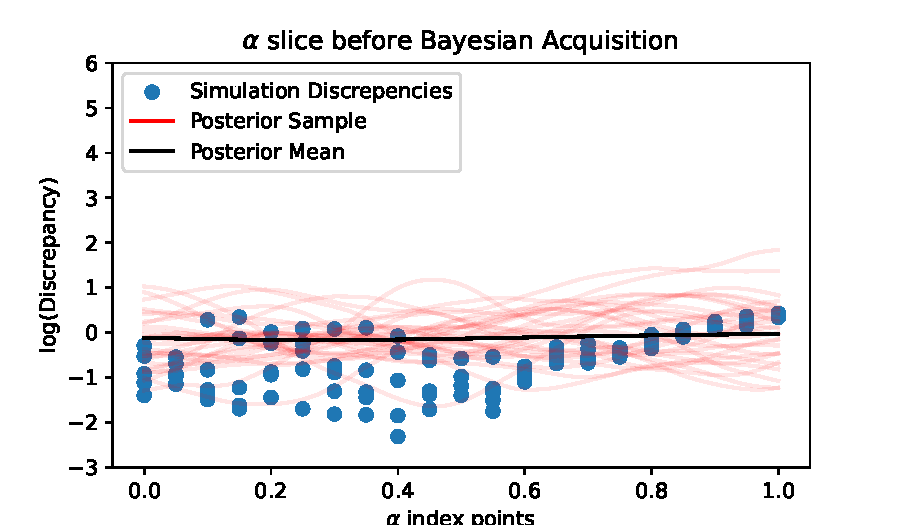
\includegraphics[width=\textwidth]{
            ../champagne_GP_images/initial_alpha_slice_log_discrep.pdf
        }
    \end{subfigure}%
    \hfill%
    \begin{subfigure}[b]{0.5\textwidth}
        \centering
        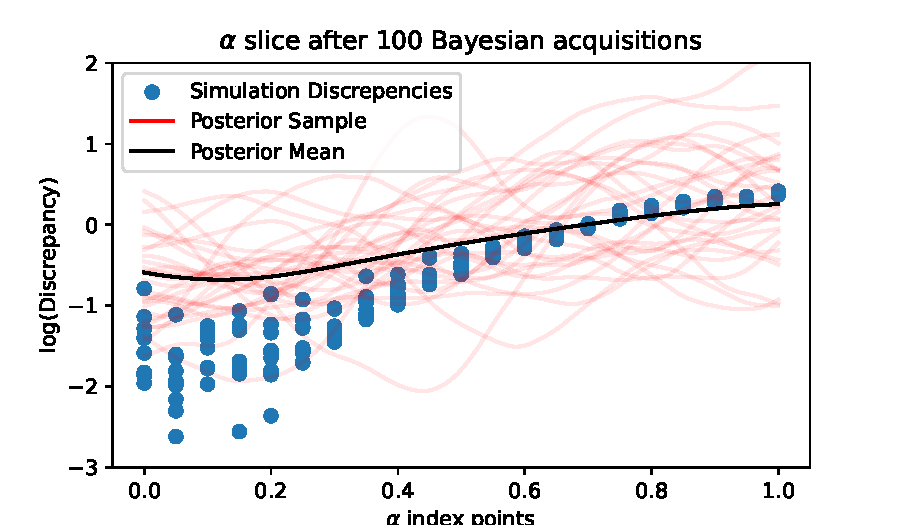
\includegraphics[width=\textwidth]{
            ../champagne_GP_images/alpha_slice_100_bolfi_updates_log_discrep.pdf
        }
    \end{subfigure}
    \hfill%
    \begin{subfigure}[b]{0.5\textwidth}
        \centering
        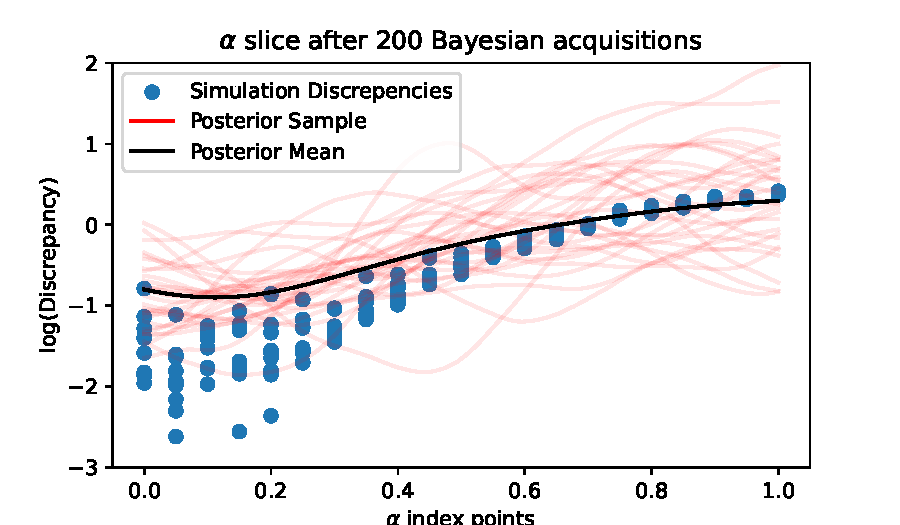
\includegraphics[width=\textwidth]{
            ../champagne_GP_images/alpha_slice_200_bolfi_updates_log_discrep.pdf
        }
    \end{subfigure}%
    \hfill%
    \begin{subfigure}[b]{0.5\textwidth}
        \centering
        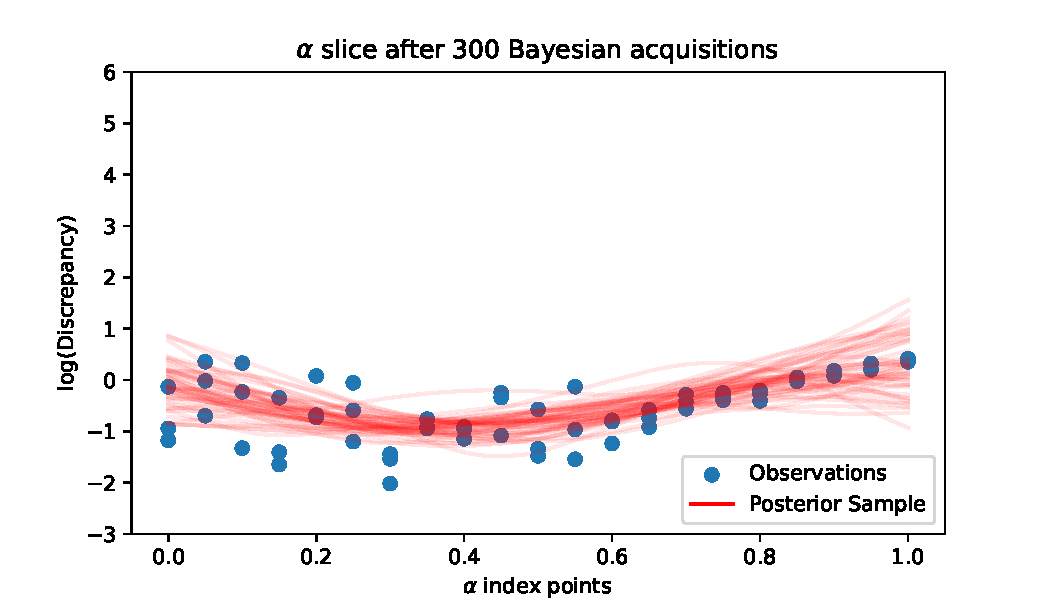
\includegraphics[width=\textwidth]{
            ../champagne_GP_images/alpha_slice_300_bolfi_updates_log_discrep.pdf
        }
    \end{subfigure}%
    \hfill%
    \begin{subfigure}[b]{0.5\textwidth}
        \centering
        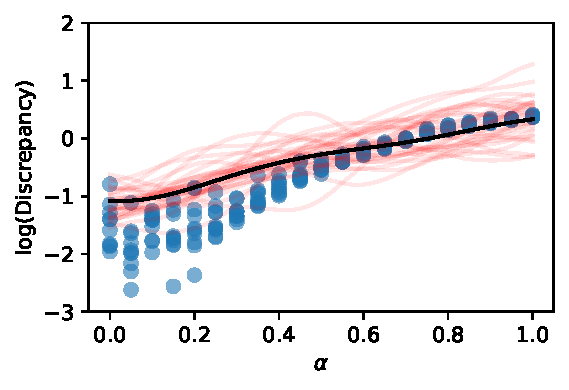
\includegraphics[width=\textwidth]{
            ../champagne_GP_images/alpha_slice_400_bolfi_updates_log_discrep.pdf
        }
    \end{subfigure}
    \caption{
        $d_\GP^{(t)}(\btheta)$ approximation of $\E(\ln\D(\btheta)),$ 
        for $t= 0$, $100$, $200$, $300$, and $400.$ Only $\alpha$ was 
        varied. All other parameters were fixed at the true values. Black line 
        is
        $\E(d^{(i)}(\btheta)).$
        Blue dots are realisations from $\ln\D(\btheta).$
    }
\end{figure}

\begin{figure}[htbp]
    \centering
    \begin{subfigure}[b]{0.5\textwidth}
        \centering
        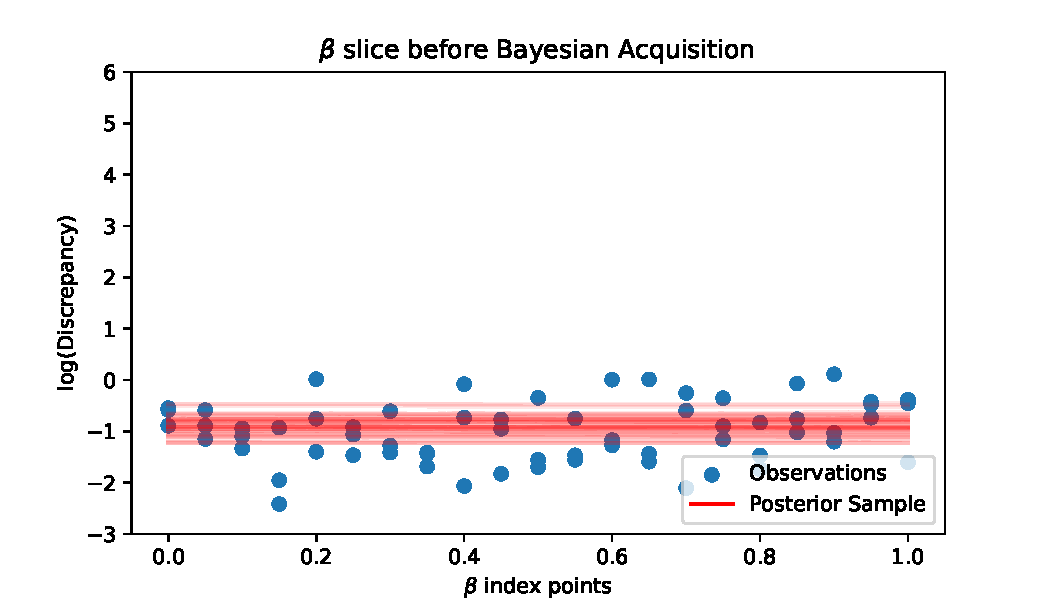
\includegraphics[width=\textwidth]{
            ../champagne_GP_images/initial_beta_slice_log_discrep.pdf
        }
    \end{subfigure}%
    \hfill%
    \begin{subfigure}[b]{0.5\textwidth}
        \centering
        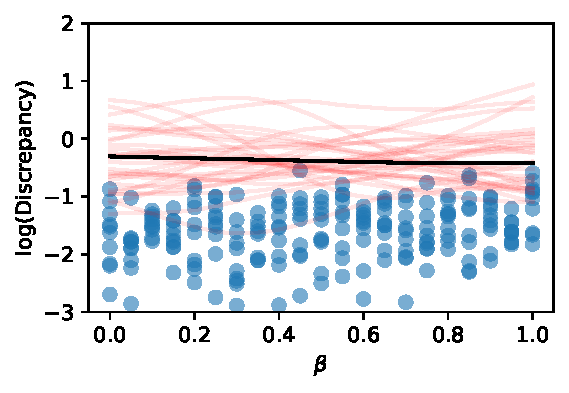
\includegraphics[width=\textwidth]{
            ../champagne_GP_images/beta_slice_100_bolfi_updates_log_discrep.pdf
        }
    \end{subfigure}
    \hfill%
    \begin{subfigure}[b]{0.5\textwidth}
        \centering
        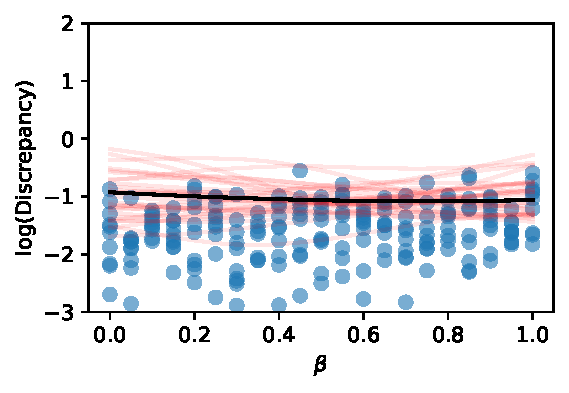
\includegraphics[width=\textwidth]{
            ../champagne_GP_images/beta_slice_200_bolfi_updates_log_discrep.pdf
        }
    \end{subfigure}%
    \hfill%
    \begin{subfigure}[b]{0.5\textwidth}
        \centering
        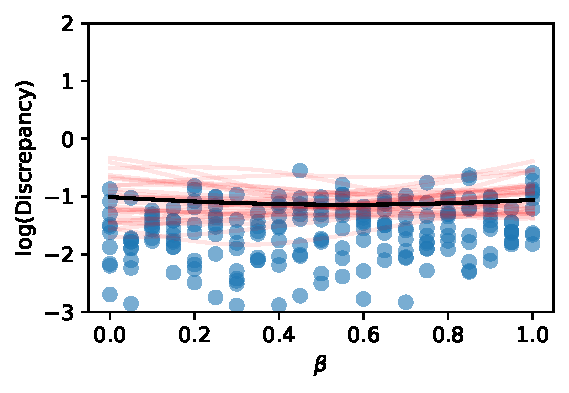
\includegraphics[width=\textwidth]{
            ../champagne_GP_images/beta_slice_300_bolfi_updates_log_discrep.pdf
        }
    \end{subfigure}%
    \hfill%
    \begin{subfigure}[b]{0.5\textwidth}
        \centering
        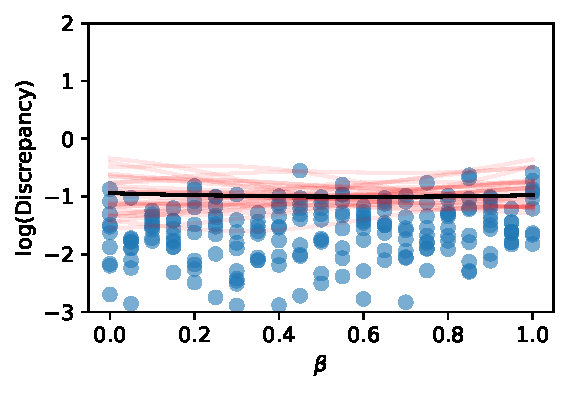
\includegraphics[width=\textwidth]{
            ../champagne_GP_images/beta_slice_400_bolfi_updates_log_discrep.pdf
        }
    \end{subfigure}
    \caption{
        $d_\GP^{(t)}(\btheta)$ approximation of $\E(\ln\D(\btheta)),$ 
        for $t= 0$, $100$, $200$, $300$, and $400.$ Only $\beta$ was 
        varied. All other parameters were fixed at the true values. Black line 
        is
        $\E(d^{(i)}(\btheta)).$
        Blue dots are realisations from $\ln\D(\btheta).$
    }
\end{figure}

\begin{figure}[htbp]
    \centering
    \begin{subfigure}[b]{0.5\textwidth}
        \centering
        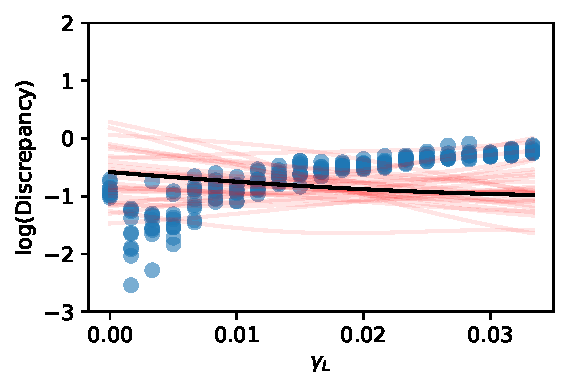
\includegraphics[width=\textwidth]{
            ../champagne_GP_images/initial_gamma_L_slice_log_discrep.pdf
        }
    \end{subfigure}%
    \hfill%
    \begin{subfigure}[b]{0.5\textwidth}
        \centering
        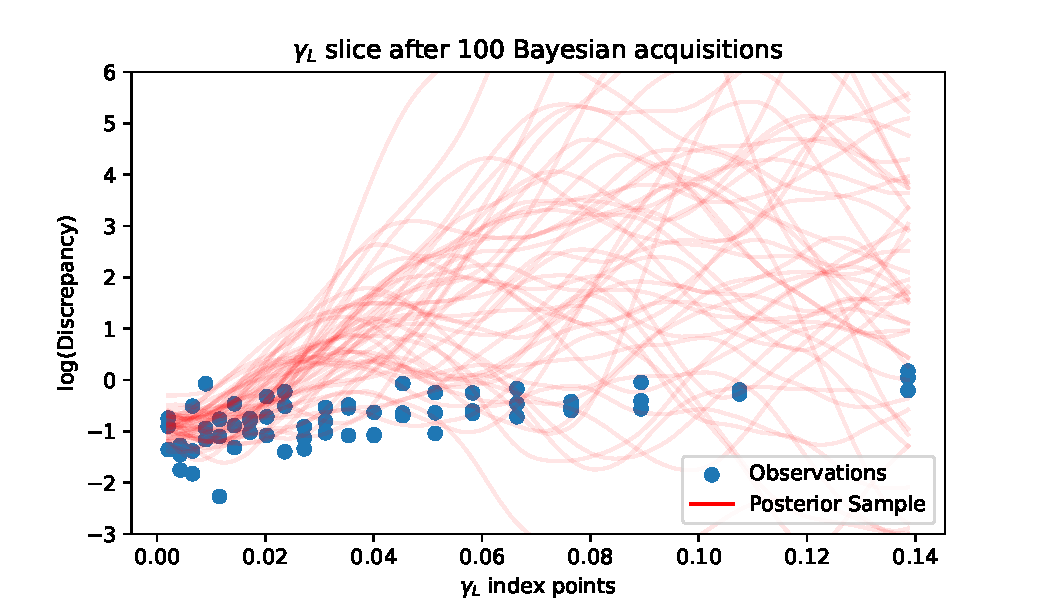
\includegraphics[width=\textwidth]{
            ../champagne_GP_images/gamma_L_slice_100_bolfi_updates_log_discrep.pdf
        }
    \end{subfigure}
    \hfill%
    \begin{subfigure}[b]{0.5\textwidth}
        \centering
        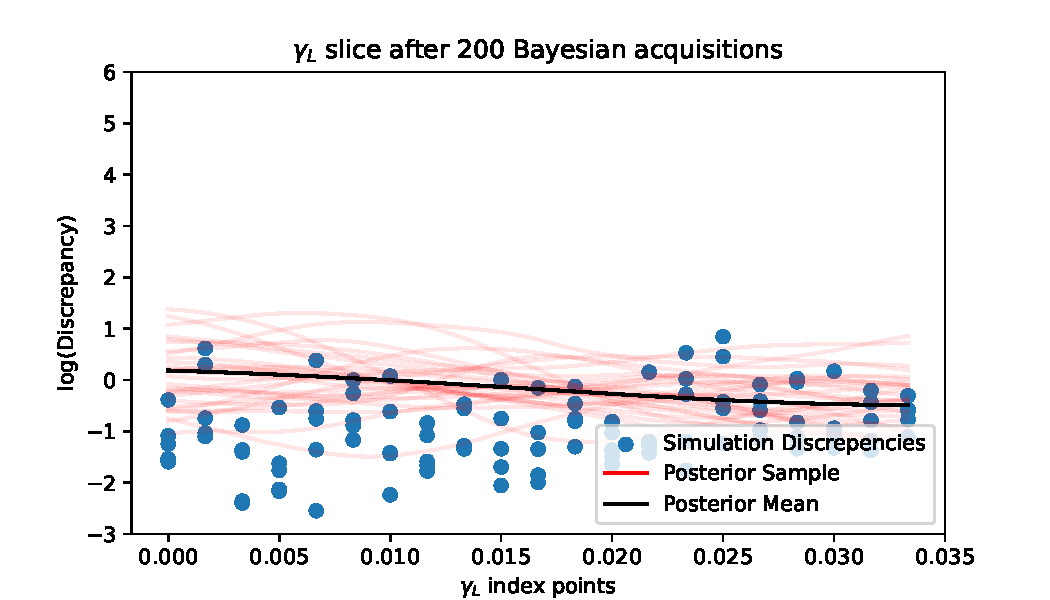
\includegraphics[width=\textwidth]{
            ../champagne_GP_images/gamma_L_slice_200_bolfi_updates_log_discrep.pdf
        }
    \end{subfigure}%
    \hfill%
    \begin{subfigure}[b]{0.5\textwidth}
        \centering
        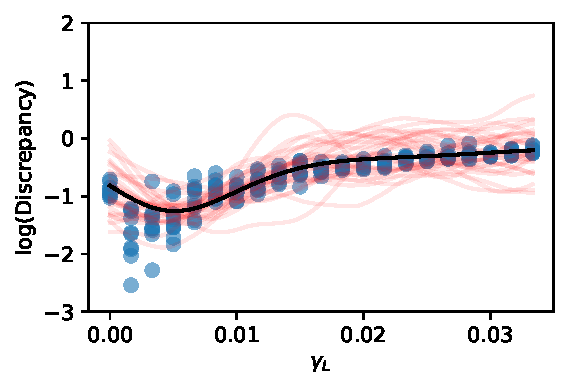
\includegraphics[width=\textwidth]{
            ../champagne_GP_images/gamma_L_slice_300_bolfi_updates_log_discrep.pdf
        }
    \end{subfigure}%
    \hfill%
    \begin{subfigure}[b]{0.5\textwidth}
        \centering
        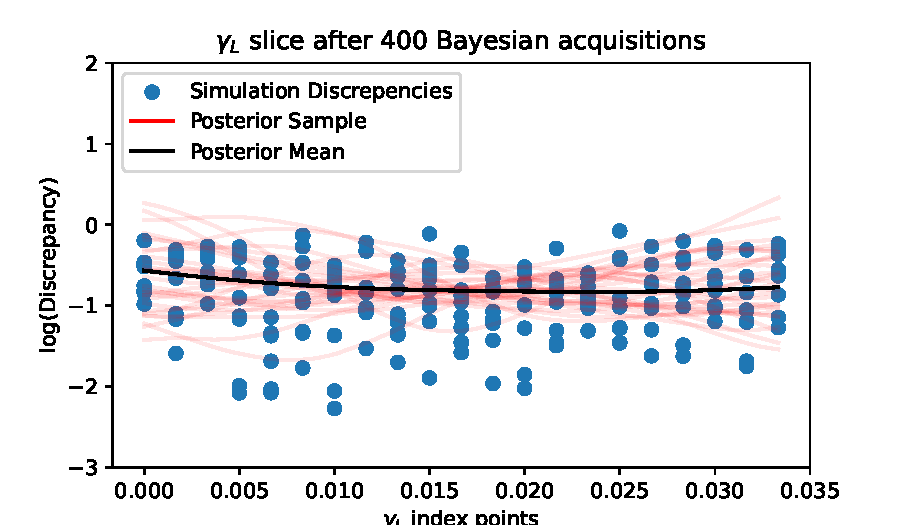
\includegraphics[width=\textwidth]{
            ../champagne_GP_images/gamma_L_slice_400_bolfi_updates_log_discrep.pdf
        }
    \end{subfigure}
    \caption{
        $d_\GP^{(t)}(\btheta)$ approximation of $\E(\ln\D(\btheta)),$ 
        for $t= 0$, $100$, $200$, $300$, and $400.$ Only $\gamma_L$ was 
        varied. All other parameters were fixed at the true values. Black line 
        is
        $\E(d^{(i)}(\btheta)).$
        Blue dots are realisations from $\ln\D(\btheta).$
    }
\end{figure}

\begin{figure}[htbp]
    \centering
    \begin{subfigure}[b]{0.5\textwidth}
        \centering
        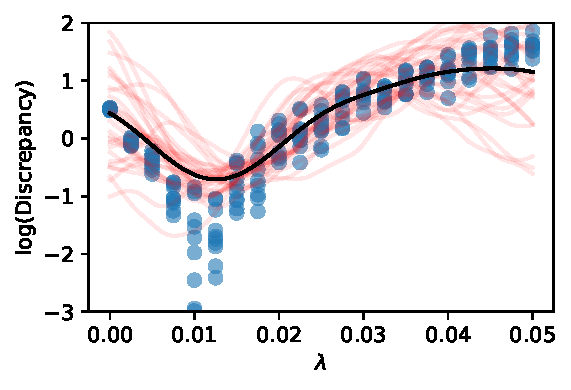
\includegraphics[width=\textwidth]{
            ../champagne_GP_images/initial_lambda_slice_log_discrep.pdf
        }
    \end{subfigure}%
    \hfill%
    \begin{subfigure}[b]{0.5\textwidth}
        \centering
        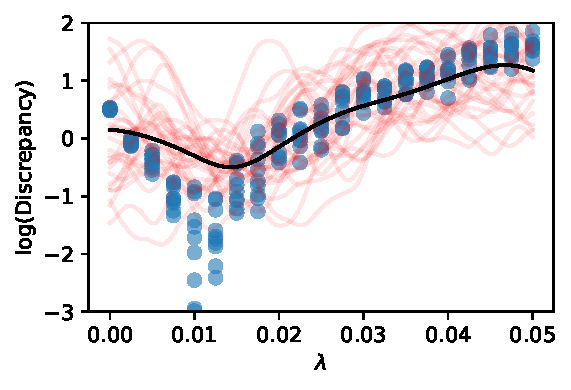
\includegraphics[width=\textwidth]{
            ../champagne_GP_images/lambda_slice_100_bolfi_updates_log_discrep.pdf
        }
    \end{subfigure}
    \hfill%
    \begin{subfigure}[b]{0.5\textwidth}
        \centering
        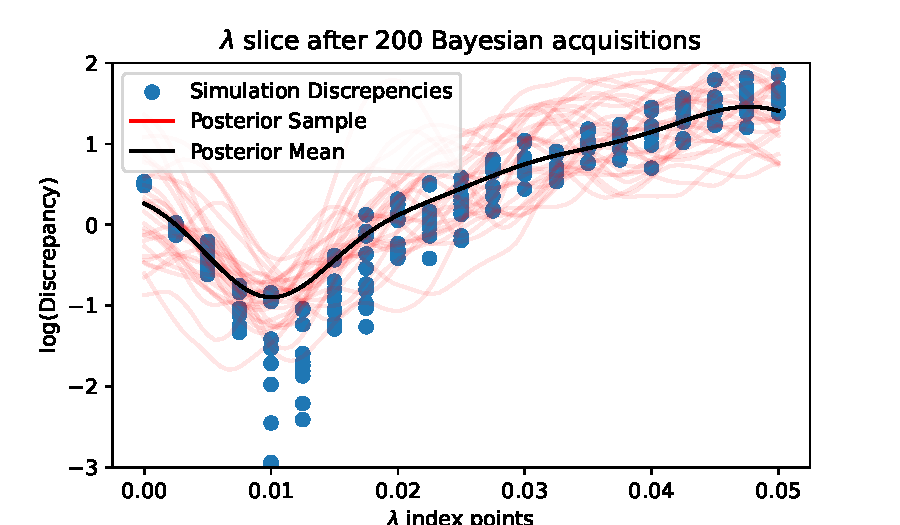
\includegraphics[width=\textwidth]{
            ../champagne_GP_images/lambda_slice_200_bolfi_updates_log_discrep.pdf
        }
    \end{subfigure}%
    \hfill%
    \begin{subfigure}[b]{0.5\textwidth}
        \centering
        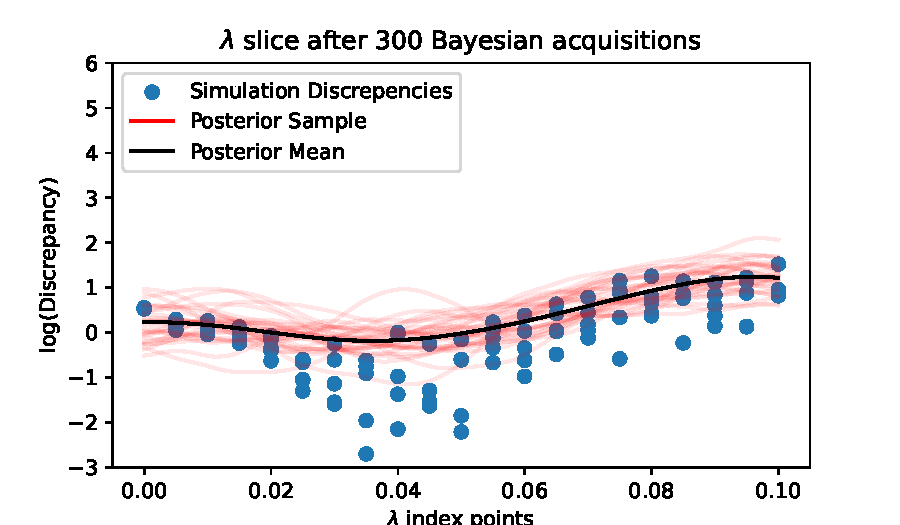
\includegraphics[width=\textwidth]{
            ../champagne_GP_images/lambda_slice_300_bolfi_updates_log_discrep.pdf
        }
    \end{subfigure}%
    \hfill%
    \begin{subfigure}[b]{0.5\textwidth}
        \centering
        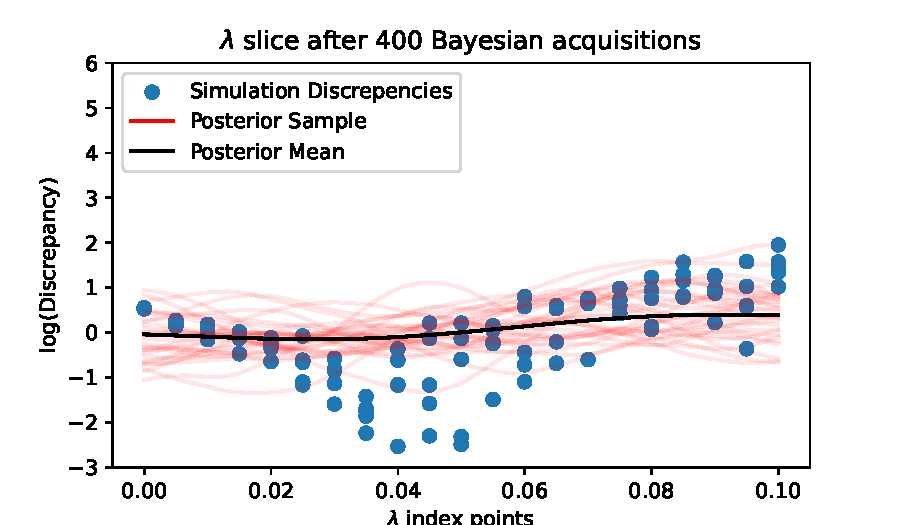
\includegraphics[width=\textwidth]{
            ../champagne_GP_images/lambda_slice_400_bolfi_updates_log_discrep.pdf
        }
    \end{subfigure}
    \caption{
        $d_\GP^{(t)}(\btheta)$ approximation of $\E(\ln\D(\btheta)),$ 
        for $t= 0$, $100$, $200$, $300$, and $400.$ Only $\lambda$ was 
        varied. All other parameters were fixed at the true values. Black line 
        is
        $\E(d^{(i)}(\btheta)).$
        Blue dots are realisations from $\ln\D(\btheta).$
    }
\end{figure}

\begin{figure}[htbp]
    \centering
    \begin{subfigure}[b]{0.5\textwidth}
        \centering
        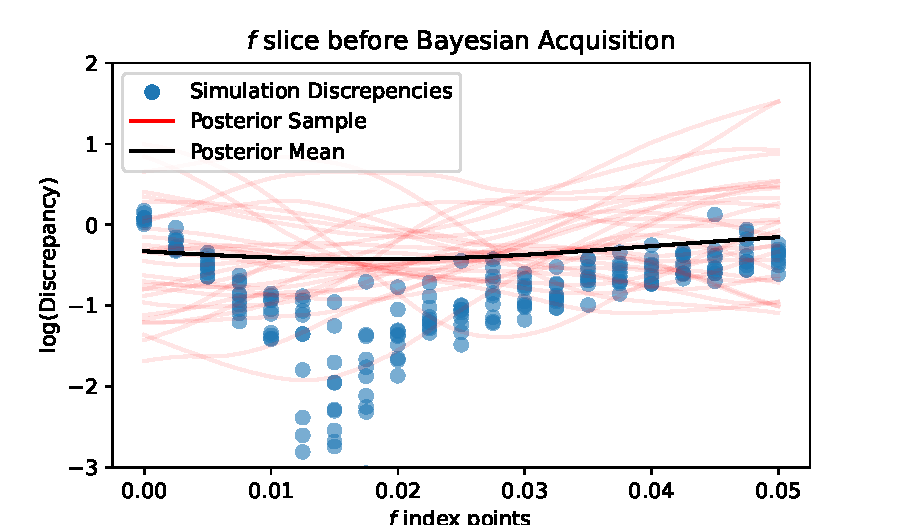
\includegraphics[width=\textwidth]{
            ../champagne_GP_images/initial_f_slice_log_discrep.pdf
        }
    \end{subfigure}%
    \hfill%
    \begin{subfigure}[b]{0.5\textwidth}
        \centering
        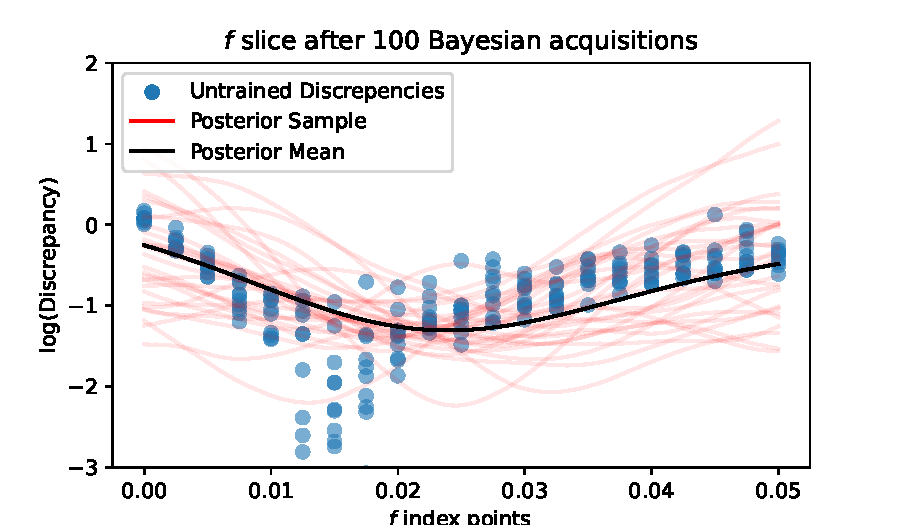
\includegraphics[width=\textwidth]{
            ../champagne_GP_images/f_slice_100_bolfi_updates_log_discrep.pdf
        }
    \end{subfigure}
    \hfill%
    \begin{subfigure}[b]{0.5\textwidth}
        \centering
        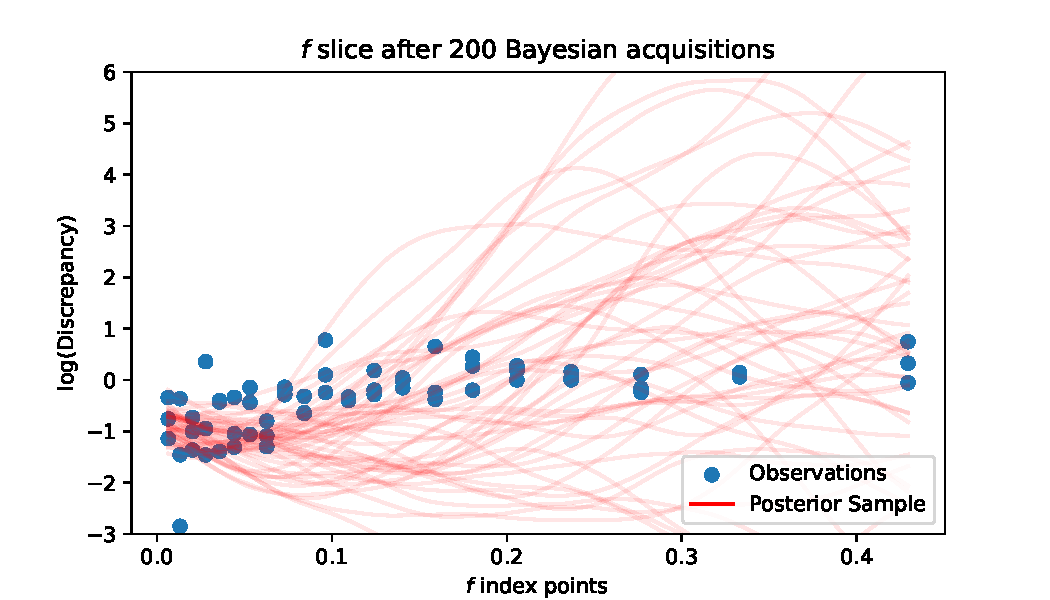
\includegraphics[width=\textwidth]{
            ../champagne_GP_images/f_slice_200_bolfi_updates_log_discrep.pdf
        }
    \end{subfigure}%
    \hfill%
    \begin{subfigure}[b]{0.5\textwidth}
        \centering
        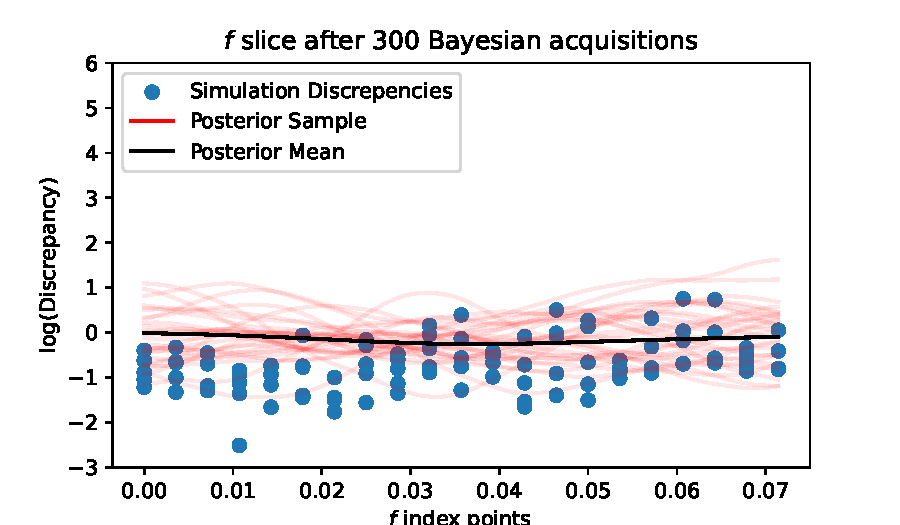
\includegraphics[width=\textwidth]{
            ../champagne_GP_images/f_slice_300_bolfi_updates_log_discrep.pdf
        }
    \end{subfigure}%
    \hfill%
    \begin{subfigure}[b]{0.5\textwidth}
        \centering
        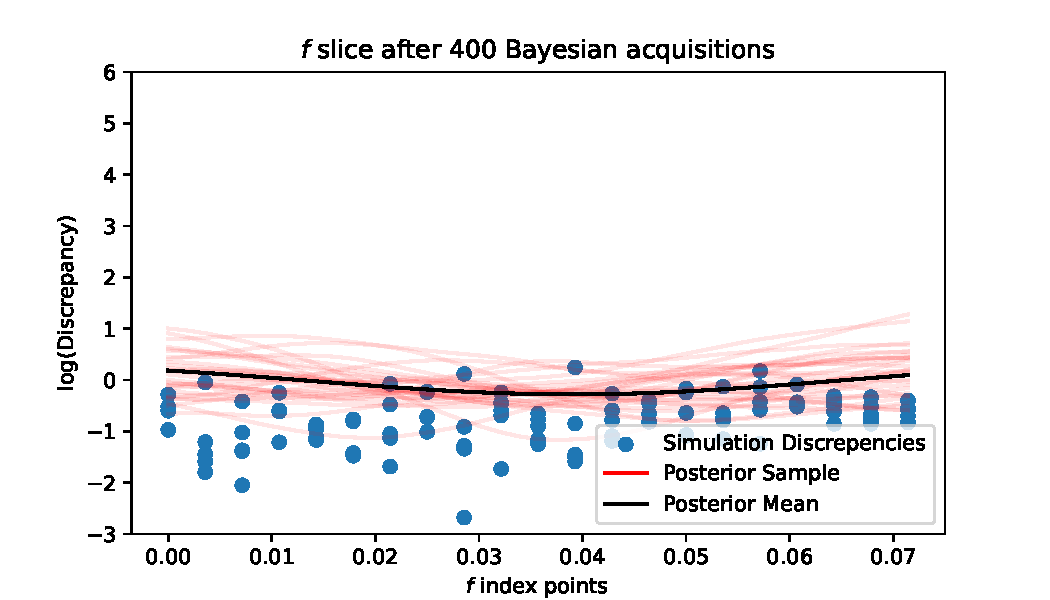
\includegraphics[width=\textwidth]{
            ../champagne_GP_images/f_slice_400_bolfi_updates_log_discrep.pdf
        }
    \end{subfigure}
    \caption{
        $d_\GP^{(t)}(\btheta)$ approximation of $\E(\ln\D(\btheta)),$ 
        for $t= 0$, $100$, $200$, $300$, and $400.$ Only $f$ was 
        varied. All other parameters were fixed at the true values. Black line 
        is
        $\E(d^{(i)}(\btheta)).$
        Blue dots are realisations from $\ln\D(\btheta).$
    }
\end{figure}

\begin{figure}[htbp]
    \centering
    \begin{subfigure}[b]{0.5\textwidth}
        \centering
        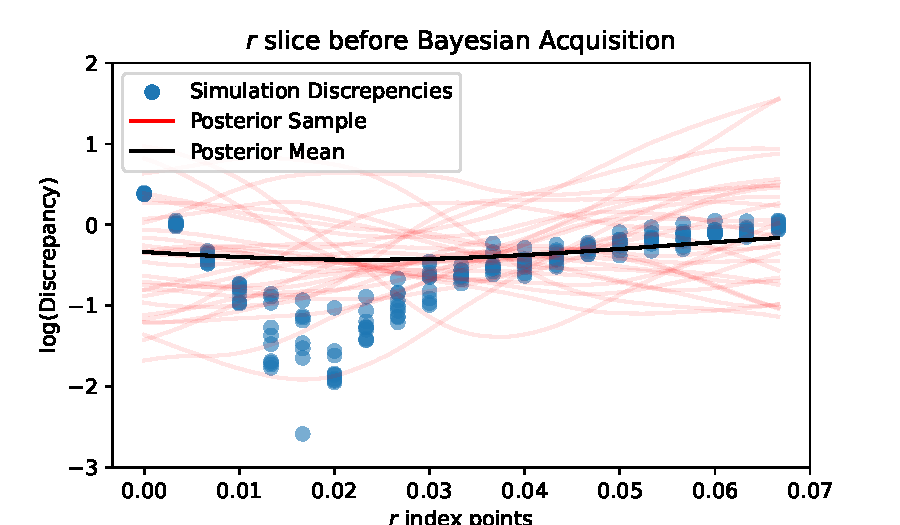
\includegraphics[width=\textwidth]{
            ../champagne_GP_images/initial_r_slice_log_discrep.pdf
        }
    \end{subfigure}%
    \hfill%
    \begin{subfigure}[b]{0.5\textwidth}
        \centering
        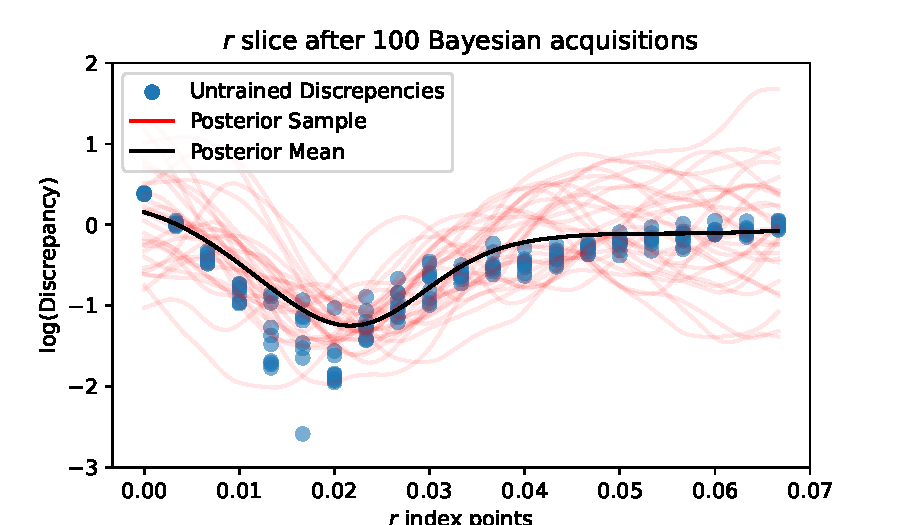
\includegraphics[width=\textwidth]{
            ../champagne_GP_images/r_slice_100_bolfi_updates_log_discrep.pdf
        }
    \end{subfigure}
    \hfill%
    \begin{subfigure}[b]{0.5\textwidth}
        \centering
        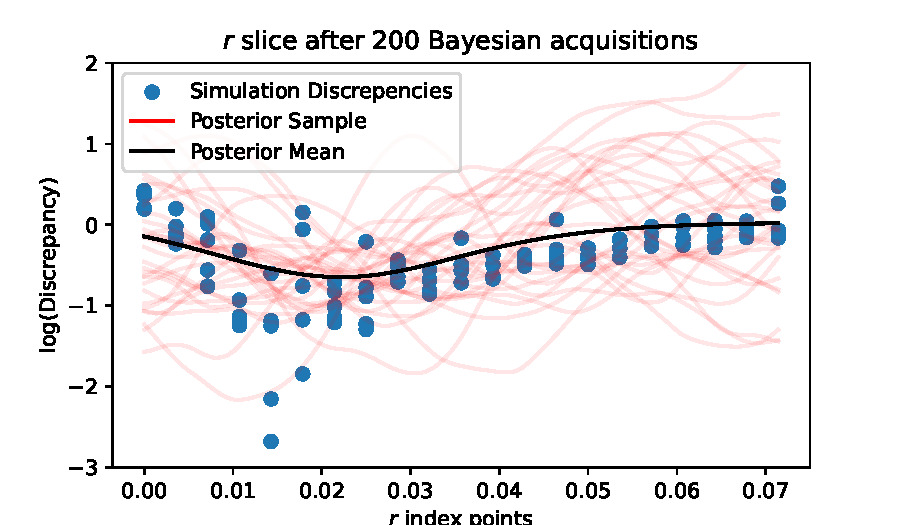
\includegraphics[width=\textwidth]{
            ../champagne_GP_images/r_slice_200_bolfi_updates_log_discrep.pdf
        }
    \end{subfigure}%
    \hfill%
    \begin{subfigure}[b]{0.5\textwidth}
        \centering
        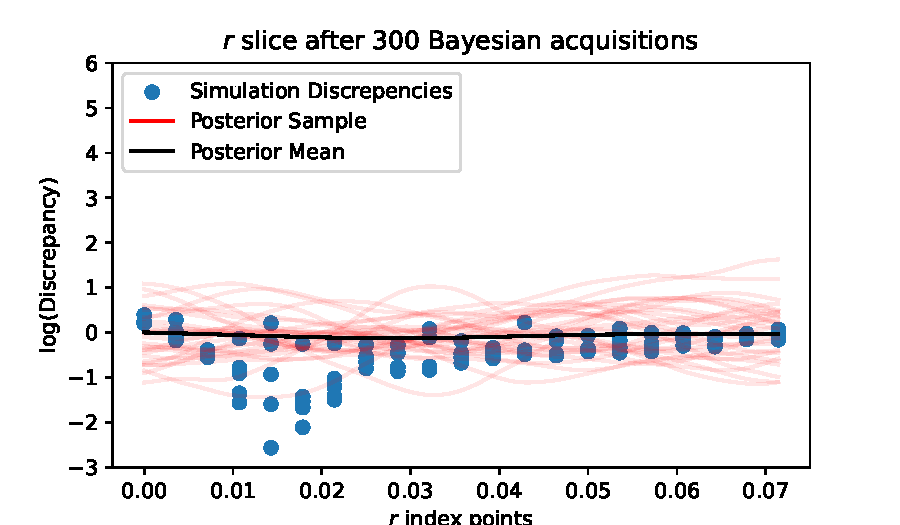
\includegraphics[width=\textwidth]{
            ../champagne_GP_images/r_slice_300_bolfi_updates_log_discrep.pdf
        }
    \end{subfigure}%
    \hfill%
    \begin{subfigure}[b]{0.5\textwidth}
        \centering
        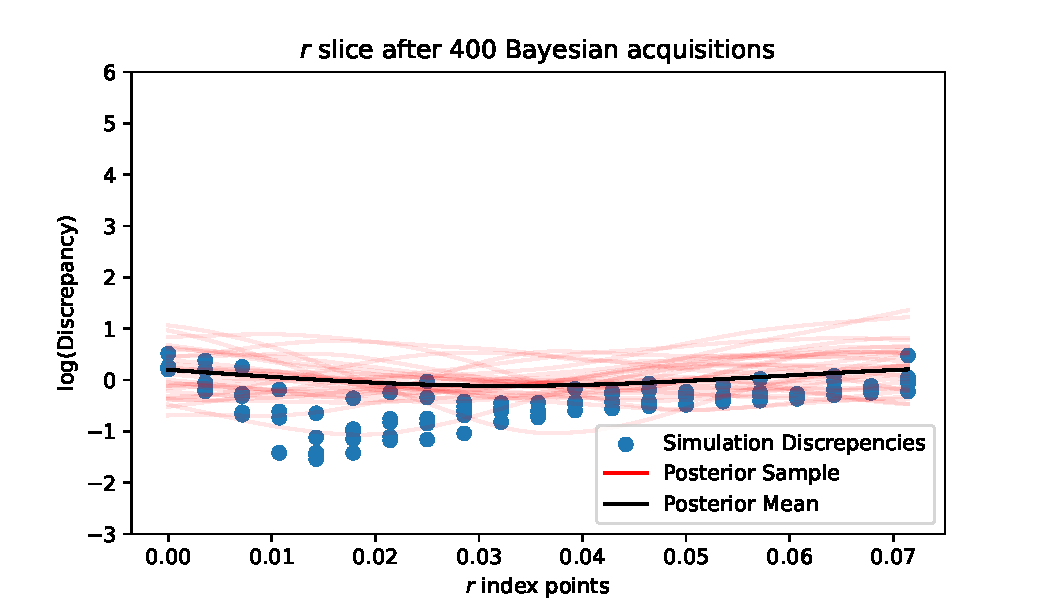
\includegraphics[width=\textwidth]{
            ../champagne_GP_images/r_slice_400_bolfi_updates_log_discrep.pdf
        }
    \end{subfigure}
    \caption{
        $d_\GP^{(t)}(\btheta)$ approximation of $\E(\ln\D(\btheta)),$ 
        for $t= 0$, $100$, $200$, $300$, and $400.$ Only $r$ was 
        varied. All other parameters were fixed at the true values. Black line 
        is
        $\E(d^{(i)}(\btheta)).$
        Blue dots are realisations from $\ln\D(\btheta).$
    }
\end{figure}